\section{Methodological Approach and Structure}
The review follows structured IS/medical literature guidance (concept
matrix inspired by \parencite{websterAnalyzingPrepareFuture2002} and PRISMA
principles \parencite{tugwellPRISMA20202021}). The methodological approach uses a multi-stage search and
transparent extraction and synthesis procedures as outlined below.

\begin{enumerate}
  \item \textbf{Search strategy (Multi-stage, 2015-2025):}
    \begin{itemize}
      \item \textbf{Scoping:} Google Scholar for broad coverage and
        identifying candidate papers.
      \item \textbf{Formal queries:} IEEE Xplore, PubMed, and Scopus
        using controlled keyword strings and deduplication.
      \item \textbf{Citation chasing:} Backward and forward citation
        tracking on key papers to ensure completeness.
    \end{itemize}
  \item \textbf{Inclusion / Exclusion criteria:}
    \begin{itemize}
      \item \textbf{Inclusion:} Studies using wearable/non-EEG autonomic
        signals for seizure detection or preictal prediction.
      \item \textbf{Exclusion:} EEG-only studies, invasive recordings,
        or papers limited to purely algorithmic simulations without
        human data.
    \end{itemize}
\end{enumerate}



Extracted dimensions populate two concept matrix tables with the following
fields:
\begin{enumerate}
  \item \textbf{Study Matrix (Table~\ref{tab:detection-matrix} for detection, Table~\ref{tab:forecasting-matrix} for forecasting):}
  \begin{itemize}
    \item Study identification (author, year)
    \item Objective (detection vs forecasting, seizure type)
    \item Design (prospective, retrospective, pseudo‑prospective, LOSO CV)
    \item Sample (participant count, seizure count)
    \item Device and sensor location
    \item Algorithm architecture
    \item Performance metrics (sensitivity, specificity, FPR)
    \item Key limitations
  \end{itemize}
  \item \textbf{Detailed Metrics Matrix (Table~\ref{tab:detection-architecture} for detection, Table~\ref{tab:forecasting-architecture} for forecasting):}
  \begin{itemize}
    \item Validation approach (independent test, cross‑validation, LOSO)
    \item Detection latency
    \item Patient‑level success rate
    \item Precision/PPV
    \item Additional clinical metrics (HMS, IoC, AUC, F1)
    \item Clinical notes
  \end{itemize}
\end{enumerate}

\noindent\textbf{Additional Extracted Dimensions:}
The following dimensions were extracted and analyzed to inform the narrative synthesis and dimensional analysis presented in Section~\ref{sec:results}, complementing the tabular comparison:
\begin{itemize}
  \item Setting (clinical vs ambulatory)
  \item Modality details (ECG/HRV, PPG, EDA, ACC)
  \item Evaluation granularity (sample‑ vs alarm‑based)
  \item Windowing specifics (window length, stride, overlap)
  \item Personalization strategies
  \item Interpretability and safety considerations
  \item Data characteristics and dataset identity
  \item Missing data handling (imputation, exclusion) and synthetic data use
  \item Inference requirements (latency, computational load, hardware)
\end{itemize}

This two‑table approach follows Webster \& Watson's concept matrix methodology \parencite{websterAnalyzingPrepareFuture2002}, balancing comprehensive data extraction with readable summary tables while enabling detailed dimensional analysis in the narrative synthesis.

\noindent\textbf{Prioritization Criteria:}
Studies including splits preserving patient-specific data, FAR/h reporting
and external or cross validation will be prioritized in the synthesis. A PRISMA-style flow diagram
will summarize and visualize screening and inclusion.

\section{Search Strategy}
\label{sec:pico-search}

\section{PICO-Based Search Methodology}
The literature search was structured using the PICO framework 
(Patient/Problem, Intervention, Comparison, Outcome) 
to identify relevant studies on deep learning for non-EEG epilepsy
detection. The following key terms were used in combination with 
Boolean operators (AND, OR, NOT):

\begin{enumerate}
    \item \textbf{P (Patient/Problem):} Epileptic seizures in need of detection or prediction.
    \begin{itemize}
        \item \textit{Keywords:} `epilepsy', `seizure', `ictal', `preictal'
        \item \textit{MeSH Terms (PubMed):} Epilepsy, Se54izures
    \end{itemize}

    \item \textbf{I (Intervention):} The diagnostic method based on wearable biosignals and deep learning.
    \begin{itemize}
        \item \textit{Biosignal Keywords:} `electrocardiogram', `ECG', `heart rate variability', `HRV', `photoplethysmography', `PPG', `electrodermal activity', `EDA', `accelerometer', `ACC'
        \item \textit{Technology Keywords:} `wearable', `wearable device'
        \item \textit{Method Keywords:} `deep learning', `machine learning', `convolutional neural network', `CNN', `long short-term memory', `LSTM', `neural network'
        \item \textit{MeSH Terms (PubMed):} Wearable Electronic Devices, Electrocardiography, Deep Learning
    \end{itemize}

    \item \textbf{C (Comparison):} The explicit exclusion of studies focused solely on electroencephalography (EEG) as the primary modality.
    \begin{itemize}
        \item \textit{Exclusion Keywords:} `EEG', `electroencephalography', `iEEG', `intracranial'
        \item \textit{Search Logic:} The \texttt{NOT} operator was applied to this group in all database searches.
    \end{itemize}

    \item \textbf{O (Outcome):} Metrics quantifying the performance of a detection or prediction system.
    \begin{itemize}
        \item \textit{Keywords:} `detection', `prediction', `sensitivity', `specificity', `false alarm rate', `FAR', `area under the curve', `AUC'
    \end{itemize}

\end{enumerate}


\subsection{Practical Filters and Reproducibility}
Consistent with the overall review scope, searches were restricted to
\textbf{2015--2025} and \textbf{journal articles} with few exceptions 
made regarding \textbf{conference proceedings}.
All database searches were documented (query string, platform, and
execution date). Results were deduplicated prior to screening.

\noindent\textbf{Note on exclusions:}
Because some non-EEG wearable studies rely on video-EEG for labeling,
EEG-related terms were used to filter \emph{EEG-only modalities}, not to
exclude studies that mention EEG solely as a reference standard.


\begin{figure}[htbp]
  \centering
  % Path is relative to the main document root (where main.tex is). `prisma.pdf` lives in the project root.
  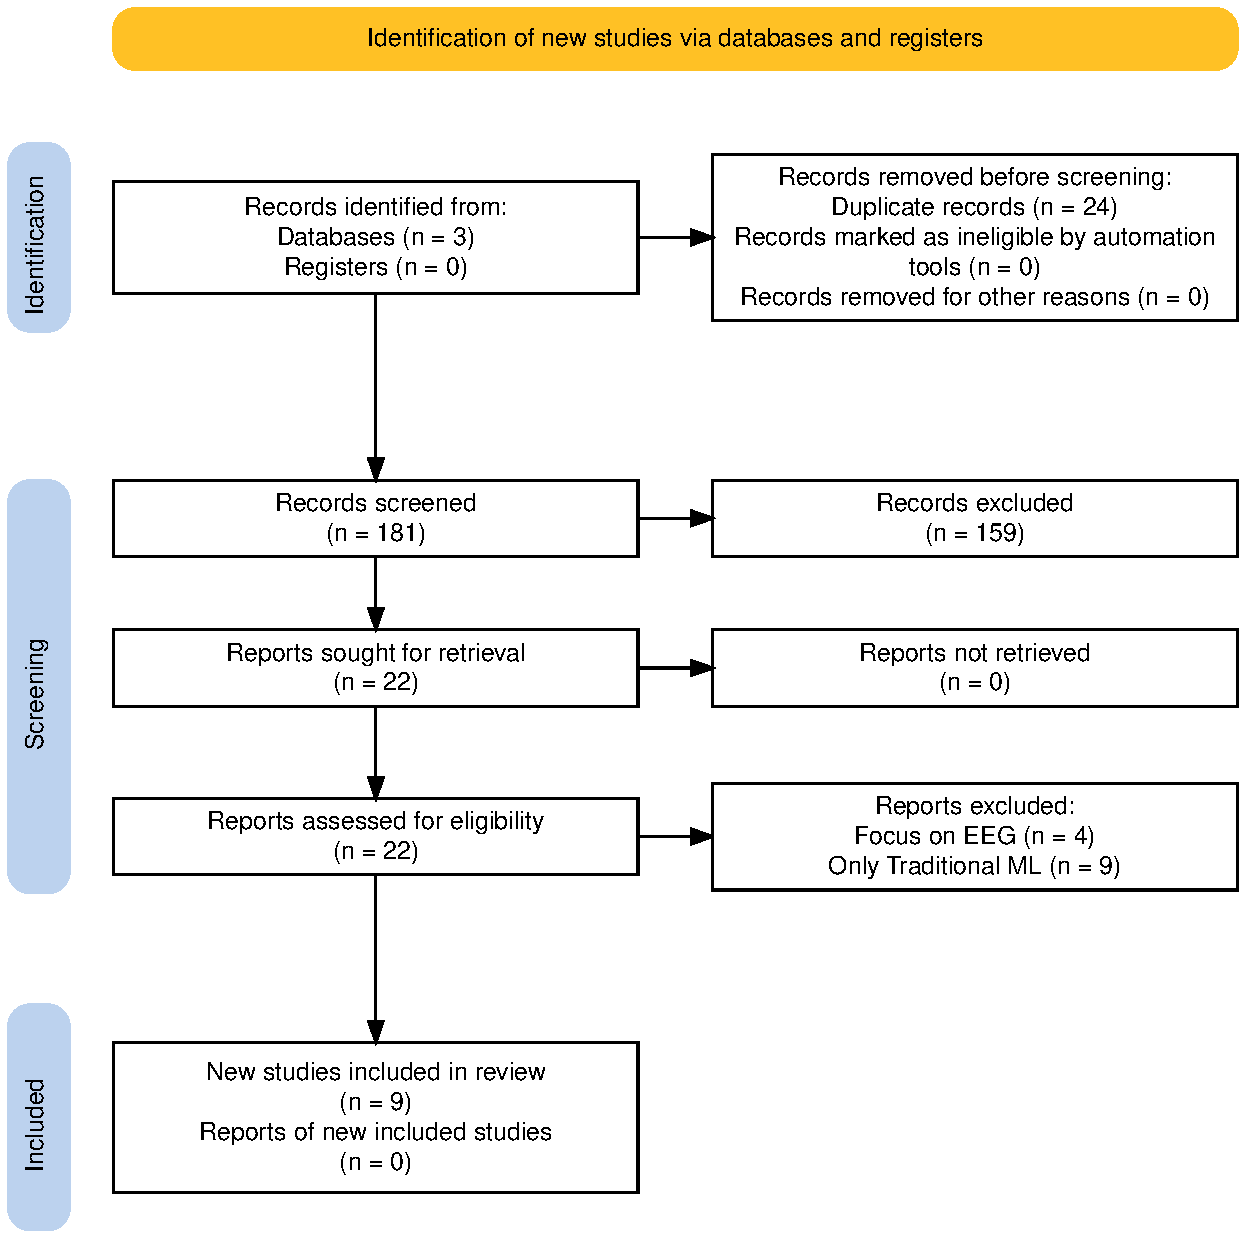
\includegraphics[width=\linewidth]{prisma.pdf}
  \caption{PRISMA flow diagram of the study selection process.}
  \label{fig:prisma}
\end{figure}